\begingroup
\setstretch{1}
\setlength{\parindent}{0pt}
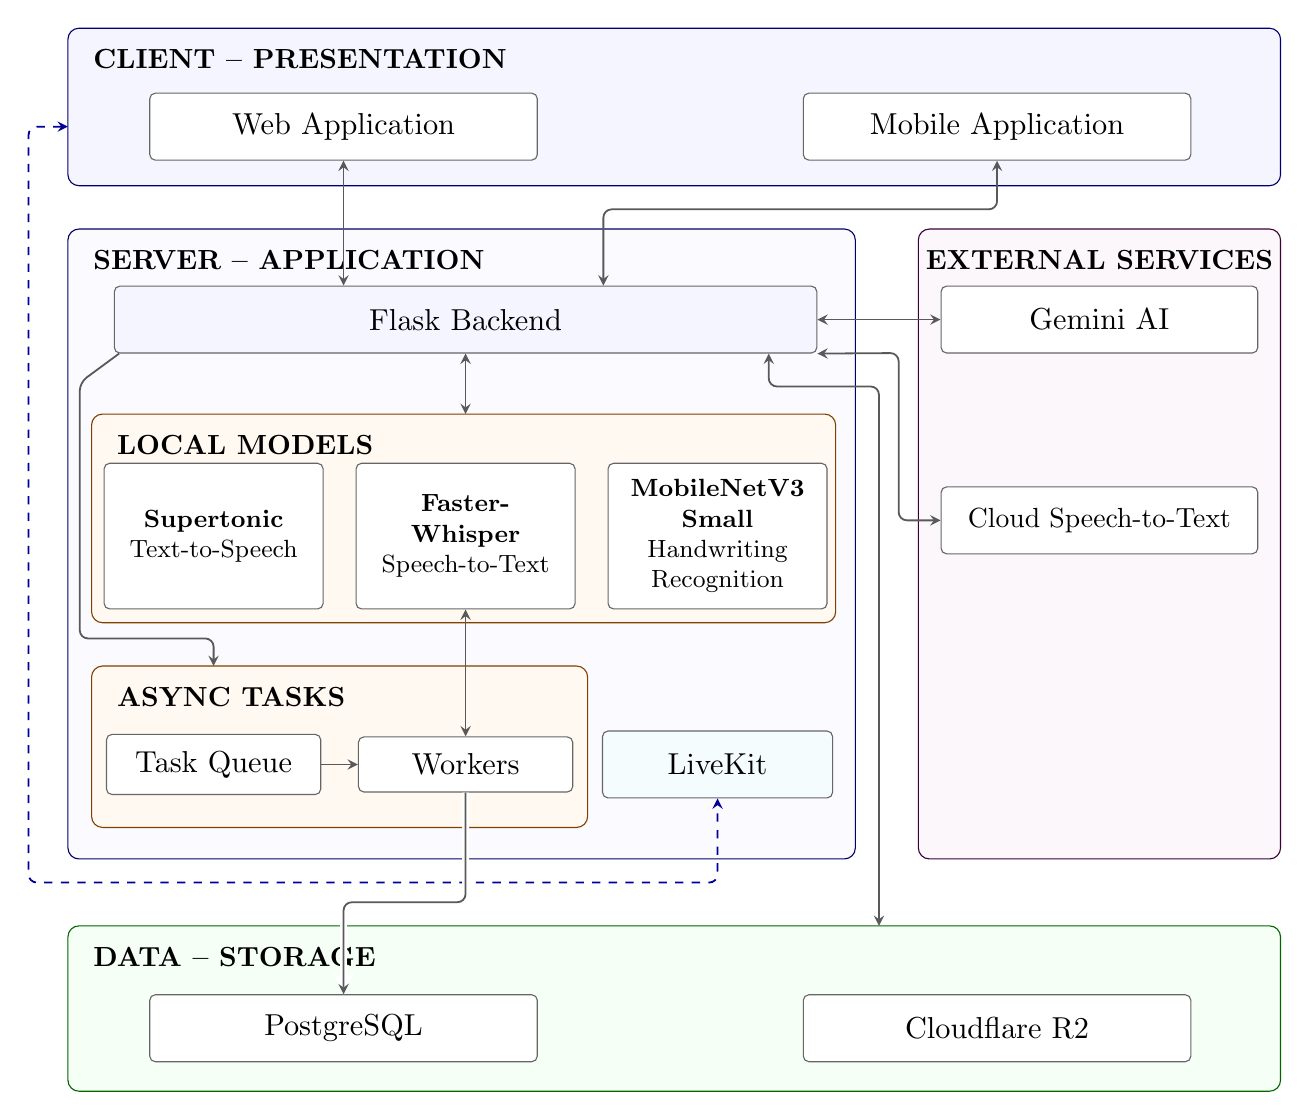
\begin{tikzpicture}[
  box/.style={draw=black!60,rounded corners=2pt,fill=white,
    text width=3.2cm,minimum height=.85cm,inner sep=6pt,
    align=center,font=\fontsize{11}{13}\selectfont},
  model/.style={box,text width=2.5cm,minimum height=1.85cm,
    font=\fontsize{9}{11}\selectfont,inner sep=4pt},
  title/.style={anchor=north west,font=\fontsize{10}{12}\selectfont\bfseries},
  link/.style={<->,>=stealth,line width=.65pt,rounded corners=3pt,draw=black!65},
  task/.style={->,>=stealth,line width=.65pt,rounded corners=3pt,draw=black!65},
  audio/.style={link,dashed,draw=blue!60!black}
]
  \draw[rounded corners,draw=blue!45!black,fill=blue!4] (-7,.9) rectangle (8.4,-1.1);
  \node[title] at (-6.8,.75) {CLIENT -- PRESENTATION};
  \node[box,text width=4.5cm] (web) at (-3.5,-.35) {Web Application};
  \node[box,text width=4.5cm] (mobile) at (4.8,-.35) {Mobile Application};

  \draw[rounded corners,draw=blue!40!black,fill=blue!2] (-7,-1.65) rectangle (3,-9.65);
  \node[title] at (-6.8,-1.8) {SERVER -- APPLICATION};
  \node[box,text width=8.5cm,fill=blue!4] (backend) at (-1.95,-2.8) {Flask Backend};
  \draw[link] (web.south) -- (web.south |- backend.north);
  \draw[link] (mobile.south) -- (4.8,-1.4) -- (-.2,-1.4) -- (-.2,0 |- backend.north);

  \draw[rounded corners,draw=orange!50!black,fill=orange!5] (-6.7,-4) rectangle (2.75,-6.65);
  \node[title] at (-6.5,-4.15) {LOCAL MODELS};
  \node[model] (tts) at (-5.15,-5.55) {\textbf{Supertonic}\\Text-to-Speech};
  \node[model] (whisper) at (-1.95,-5.55) {\textbf{Faster-Whisper}\\Speech-to-Text};
  \node[model] (kanji) at (1.25,-5.55) {\textbf{MobileNetV3}\\\textbf{Small}\\Handwriting\\Recognition};
  \draw[link] (backend.south) -- (-1.95,-4);

  \draw[rounded corners,draw=orange!50!black,fill=orange!5] (-6.7,-7.2) rectangle (-.4,-9.25);
  \node[title] at (-6.5,-7.35) {ASYNC TASKS};
  \node[box,text width=2.3cm,minimum height=.7cm] (queue) at (-5.15,-8.45) {Task Queue};
  \node[box,text width=2.3cm,minimum height=.7cm] (workers) at (-1.95,-8.45) {Workers};
  \draw[task] (queue.east) -- (workers.west);
  \draw[task] (-6.35,0 |- backend.south) -- (-6.85,-3.6) -- (-6.85,-6.85) -- (-5.15,-6.85) -- (-5.15,-7.2);
  \draw[link] (workers.north) -- (whisper.south);

  \node[box,text width=2.5cm,fill=cyan!4] (livekit) at (1.25,-8.45) {LiveKit};
  \draw[audio] (-7,-.35) -- (-7.5,-.35) -- (-7.5,-9.95) -- (1.25,-9.95) -- (livekit.south);

  \draw[rounded corners,draw=violet!45!black,fill=violet!3] (3.8,-1.65) rectangle (8.4,-9.65);
  \node[title,anchor=north] at (6.1,-1.8) {EXTERNAL SERVICES};
  \node[box,text width=3.6cm] (ai) at (6.1,-2.8) {Gemini AI};
  \node[box,text width=3.6cm,font=\fontsize{10}{12}\selectfont] (stt) at (6.1,-5.35) {Cloud Speech-to-Text};
  \draw[link] (backend.east) -- (ai.west);
  \draw[link] (backend.south east) -- (3.55,-3.225) -- (3.55,-5.35) -- (stt.west);

  \draw[rounded corners,draw=green!40!black,fill=green!4] (-7,-10.5) rectangle (8.4,-12.6);
  \node[title] at (-6.8,-10.65) {DATA -- STORAGE};
  \node[box,text width=4.5cm] (db) at (-3.5,-11.8) {PostgreSQL};
  \node[box,text width=4.5cm] (r2) at (4.8,-11.8) {Cloudflare R2};
  \draw[link] (1.9,0 |- backend.south) -- (1.9,-3.65) -- (3.3,-3.65) -- (3.3,-10.5);
  \draw[task,preaction={draw=white,line width=2.5pt}] (workers.south) -- (-1.95,-10.2) -- (-3.5,-10.2) -- (db.north);
\end{tikzpicture}
\endgroup
